\section{Experiments}
\begin{figure*}[t]
\subfigure[Implements of Restart Policy with $threshold$ settled as $128$] { \label{fig:a} 
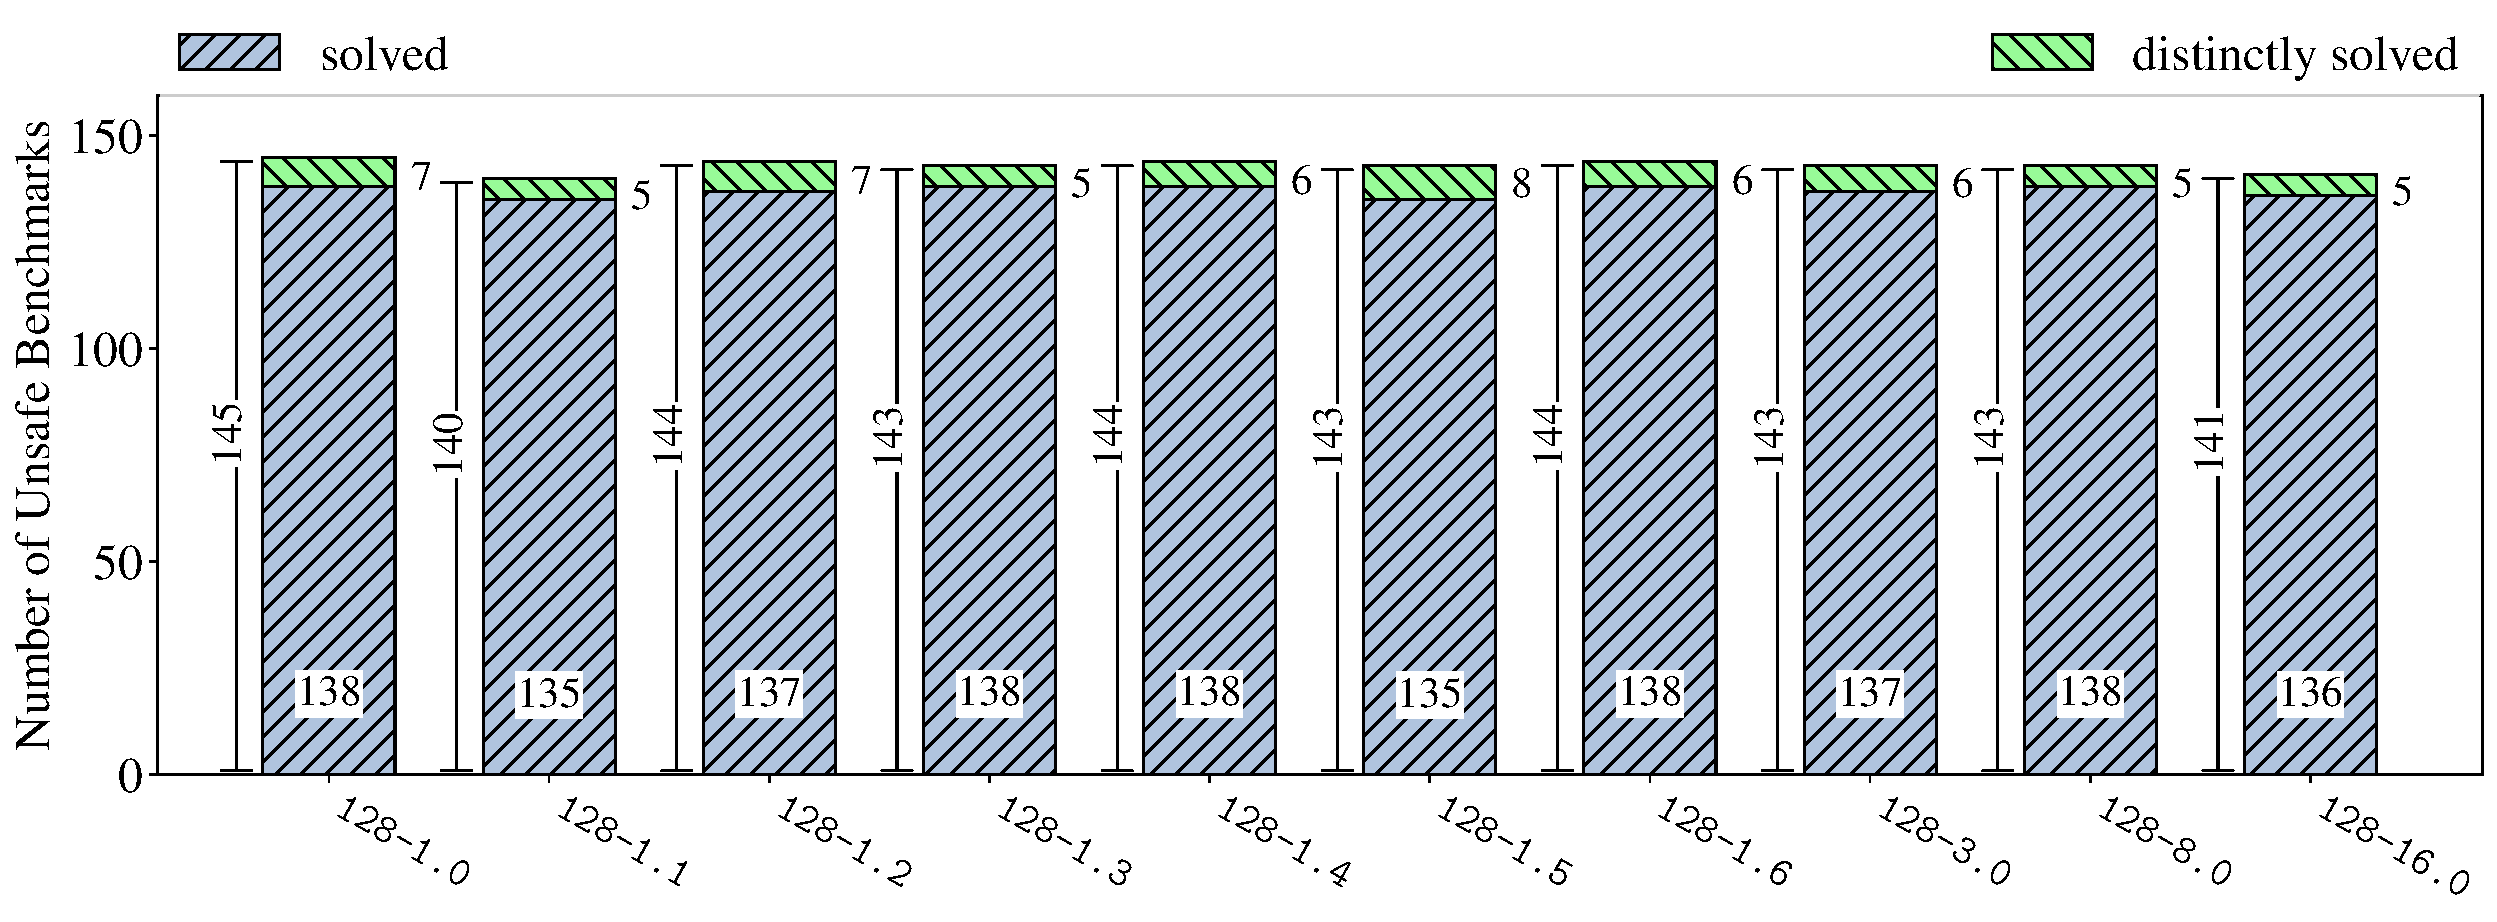
\includegraphics[width=0.49\linewidth]{images/128.pdf} 
}
\subfigure[Implements of Restart Policy with $gr$ settled as $1.0$] { \label{fig:b} 
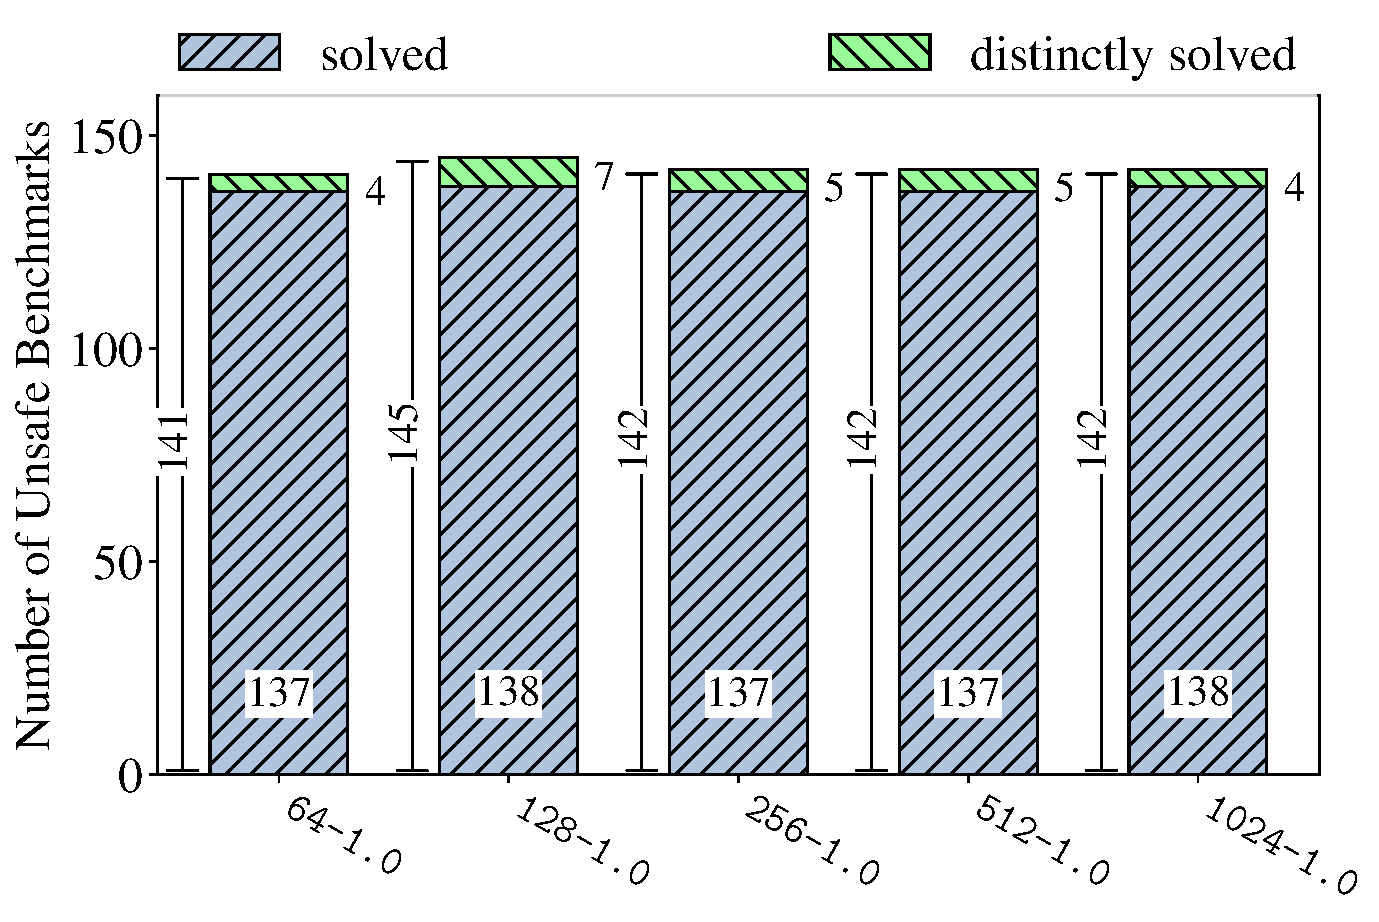
\includegraphics[width=0.49\linewidth]{images/1.0.pdf} 
}
\subfigure[Implements of Restart Policy with $gr$ settled as $1.2$] { \label{fig:c} 
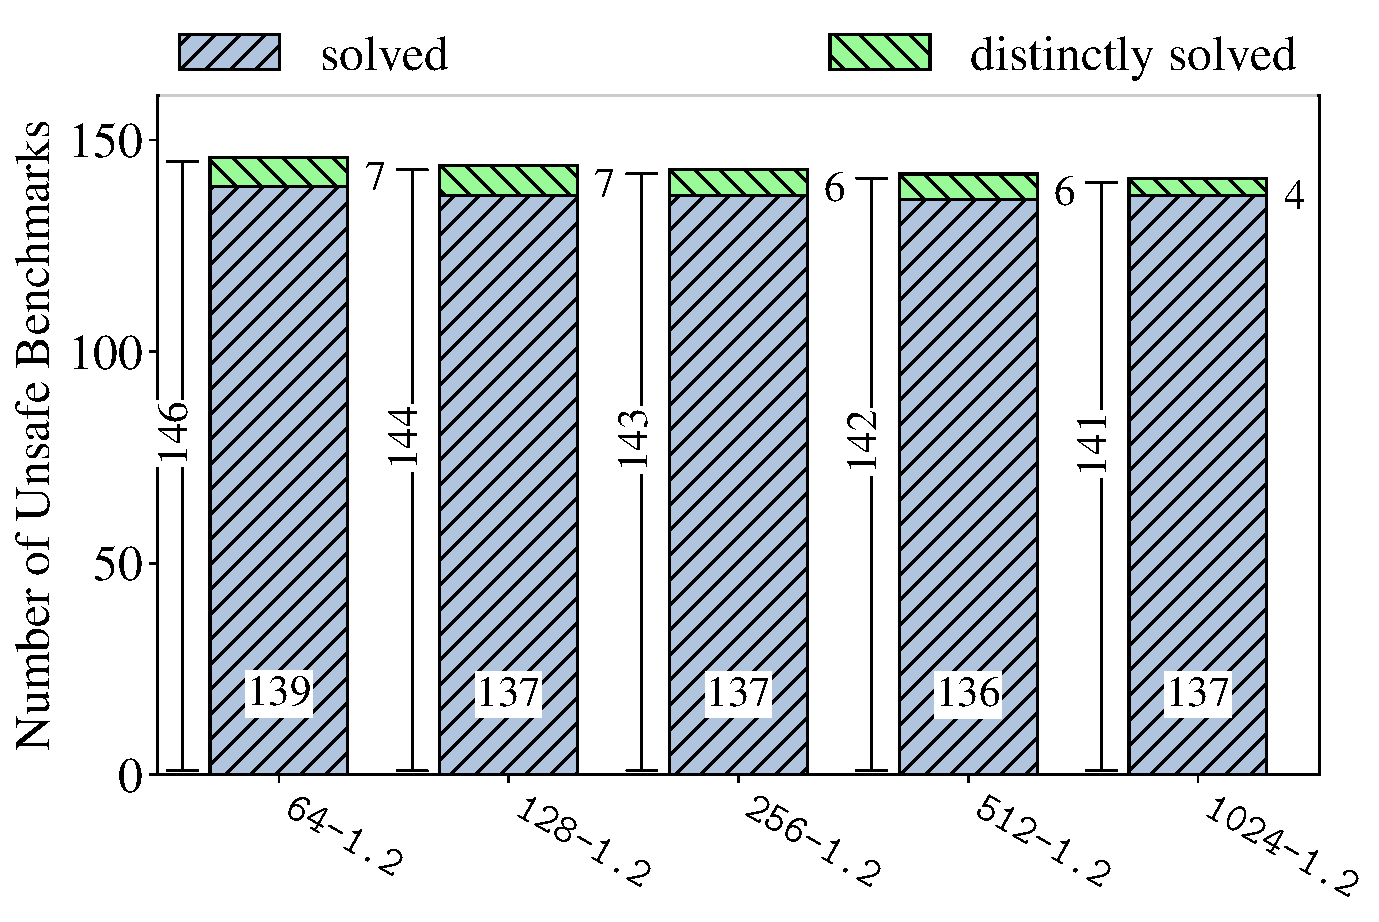
\includegraphics[width=0.49\linewidth]{images/1.2.pdf} 
}
\subfigure[Implements of Restart Policy with $gr$ settled as $1.5$] { \label{fig:d} 
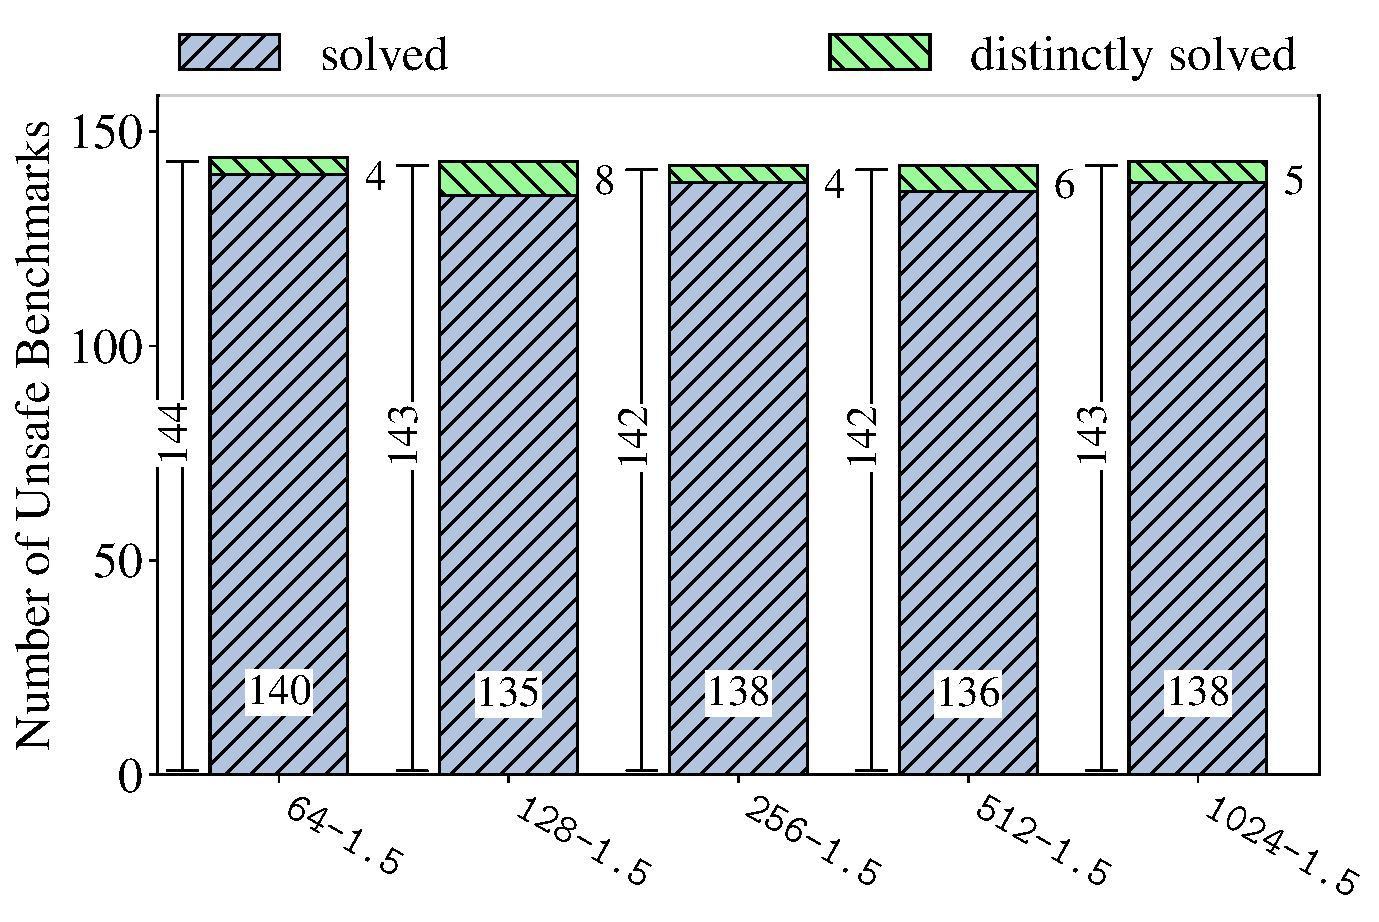
\includegraphics[width=0.49\linewidth]{images/1.5.pdf} 
}
\caption{Number of unsafe benchmarks solved by CAR after applying the restart policy. The category ``distinctly solved'' benchmarks are solved only by CAR with the restart policy. The ``solved'' benchmarks solved by CAR with and without the restart policy. X-axis 128-1.0 means $threshold=128$, $gr=1.0$ and the same applies to others.}
\end{figure*}
\subsection{Experimental Setup}
We implement the restart policy to the SimpleCAR model checker \cite{}. As mentioned before, the restart frequency has a significant influence on the effectiveness of the restart policy. In our conjecture, the frequent restarts in CAR may not preserve the advantages already achieved, while a low frequency of the algorithm cannot help solve new instances. In our proposed algorithm, two parameters $threshold$ and $gr$ are introduced to determine the restart frequency in a dynamic way. We evaluate different combinations of these two parameters. We assign a relatively small value to $threshold$ and assign $gr$ a value equal to or greater than 1 to $gr$, i.e., $threshold = 128, gr = 1.2$, aiming to avoid the disadvantage of frequent restarts by gradually increasing the threshold after each restart. 

We compare our results to those from the original CAR implemented in SimpleCAR, as well as from BMC and PDR that are integrated in ABC tool \cite{}, which is a prestigious model checker in the community and won the hardware model checking competition many times. Notably, there are kinds of BMC implementations in ABC, and we select the \emph{bmc2} which has the better performance based on previous evaluations \cite{}. Both SimpleCAR and ABC use the Minisat SAT solver \cite{} as the computation engine for model checking. 

All the experiments are performed on a cluster consisting of 2304 processor cores in 192 nodes running REDHat 6.0 with a 2.83GHz CPU and 48GB of memory (RAM). In the experiments, the time limit is set to be one hour and the memory-use is 8 GB, for each instance.
We evaluate all algorithms against 749 industrial benchmarks from the single safety property track (SINGLE) of the HWMCC in 2015 \cite{} and 2017 \cite{}. Each instance in the benchmark is an aiger model, which formalizes the And-Invertor Graph \cite{} of a circuit together with the safety property to be verified. 

This paper focuses on unsafe checking, under which a counterexample can be output to help identify the property violation. We use the aigsim tool from the Aiger package \cite{} to check whether the produced counterexamples are correct. We report that all the counterexamples generated from all checkers pass the test from aigsim.

\subsection{Results}

\subsubsection{Performance of CAR}
CAR can find \textbf{145} counterexamples before we apply the restart policy.
To evaluate the performance of the restart policy on CAR from this paper, we first set $threshold$ settled as $128$ and compare the performance of different growth rate $gr$. We display these results in \textbf{Fig. 1. (a)}, focusing on the number of instances with counterexamples, especially the new instances with a counterexample that the CAR(without restart policy) can not find. The first observation we get from the result is that the restart policy effectively expands the algorithm's diversity by finding considerable new counterexamples. In view of the fact that the restart strategy has better results when the $gr$ are 1.0, 1.2 or 1.5 from \textbf{Fig. 1.(a)} with 7 or 8 new instances, we will then set $gr$ to 1.0, 1.2 and 1.5 in other experiments.
\begin{figure}[!t]
\centering
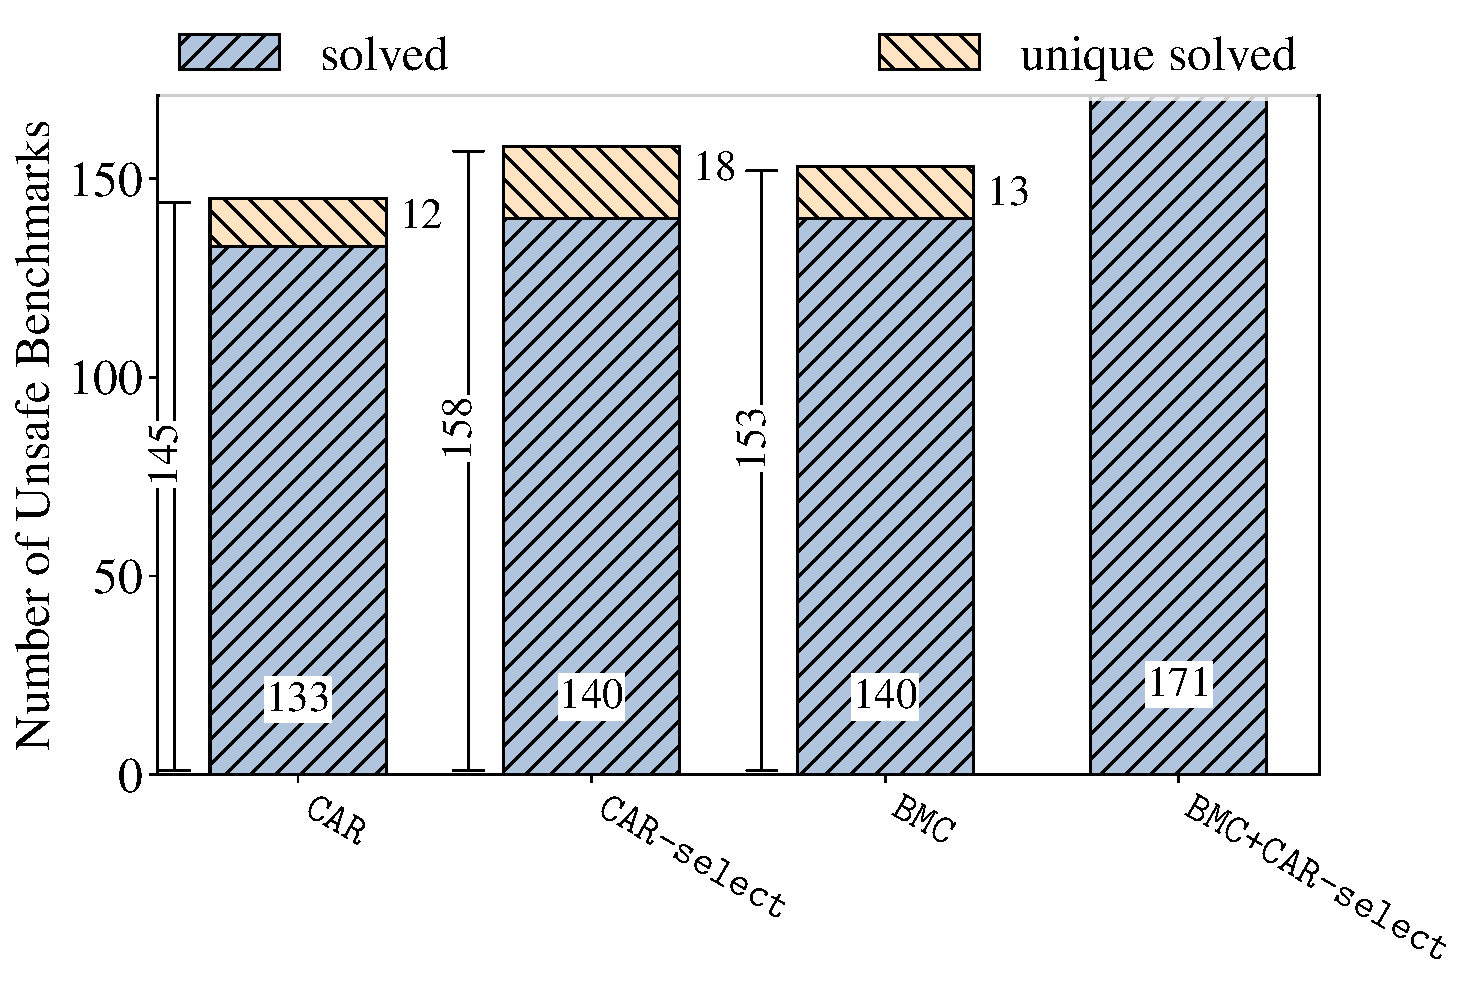
\includegraphics[width=\linewidth]{images/car-bmc.pdf} 
\caption{Number of unsafe benchmarks solved. The “uniquely solved” benchmarks are not solved by any other algorithm category, except the comparison of CAR and CAR-all.}\label{fig:compare}
\end{figure}
After observing the results from \textbf{Fig. 1. (a)}. It seems to be roughly random about how many new instances can be solved with different $gr$ from 1.0 to 1.6 and $threshold$ settled to 128. Synthesizing results from \textbf{Fig. 1. (b)(c)(d)}, restart policy performs better when the value of $threshold$ is around 128. In this interval, not only we get more ``distinctly solved'', but also several unique instances are found. For example, ``oski15a08b15s'' can only be found by ``64-1.2'',``6s351rb15'' can only be solved by ``128-1.2'' and ``oc8051topo08'' can only be solved by ``128-1.5''. Setting $threshold$ to a value of 1024 seems to be too large for a one-hour experiment to make the restart strategy work as it should be. For PDR, different given parameters will randomly lead to solving different verified-safe instances. Similarly, restart policy enables CAR to find out different bugs by using different parameters, which eventually leads to a boost in the ability of bug-finding.

\subsubsection{Comparison to original CAR and BMC }
As shown in Fig. \ref{fig:compare}, the BMC implementation in ABC solve 153 unsafe instances. CAR-all includes the results from CAR with and without the restart policy by choosing different parameters ($threshold$ and $gr$). In summary, the restart policy helps CAR find 12 more counterexamples (from 145 to 157) and 4 more ``unique solved'' that can only solved by CAR. Also, CAR-all solves 157 instances in total, which outperforms BMC (the amount is 153) and gains 15 instances that can not be found by BMC. The virtual combination of CAR-all and BMC  solves 170 instances, which affirms that the restart policy plays a non-negligible role as a part of the portfolio for hardware model checking.
